\section{Kontextabgrenzung und Systemabgrenzung}

Die Kontextabgrenzung zeigt EduPlanner in seinem Umfeld: welche Nutzer, Nachbarsysteme und externe Dienste mit dem System interagieren und über welche Schnittstellen. Die \textbf{Systemabgrenzung} (neu in arc42~v9) beschreibt explizit, was \emph{nicht} Teil des Systems ist.

\subsection{Fachlicher Kontext}

EduPlanner als Blackbox mit seinen Akteuren und Nachbarsystemen (\emph{Diagrammtyp: C4 Context Diagram}):

\begin{tabularx}{\textwidth}{L{3.2cm} L{2.8cm} X}
  \rowcolor{tableheader}
  \color{white}\textbf{Akteur / System} &
  \color{white}\textbf{Kanal} &
  \color{white}\textbf{Interaktion} \\

  Teilnehmer &
  HTTPS (Browser) &
  Self-Service-Portal: Kursübersicht, Einschreibung,
  Stornierung, Einschreibungshistorie \\

  \rowcolor{tablegrey}
  Trainer &
  HTTPS (Browser) &
  Ansicht eigener Durchführungen, Teilnehmerlisten \\

  Staff &
  HTTPS (Browser) &
  Kurs- und Durchführungsverwaltung,
  Trainer-Zuweisung \\

  \rowcolor{tablegrey}
  Admin &
  HTTPS (Browser) &
  Vollständige Verwaltungsoberfläche inkl.\
  Veröffentlichung und Nutzerverwaltung \\

  E-Mail-Dienst\footnotemark{} &
  SMTP / HTTPS &
  Transaktionaler E-Mail-Versand
  (z.\,B.\ Einschreibungsbestätigungen,
  Stornierungen, Erinnerungen) über einen
  Cloud-E-Mail-Dienst wie Amazon SES
  oder SendGrid. \\

  \rowcolor{tablegrey}
  Identity Provider (OIDC) &
  OAuth~2.0 / OIDC &
  Authentifizierung und Token-Ausstellung;
  EduPlanner verwaltet keine Passwörter. \\

  Kalender (iCal, opt.) &
  iCal / CalDAV &
  Optionaler Export in externe Kalender
  (Google, Outlook). Begründung ``optional'':
  kein Kernprozess; Implementierung in
  v1.1 geplant. \\
\end{tabularx}

\footnotetext{%
  \textbf{Amazon SES -- Simple Email Service.}
  Ein verwalteter Cloud-Dienst von AWS für den
  skalierbaren Versand transaktionaler E-Mails.
  SES übernimmt Zustellung, Bounce-Handling und
  Reputationsmanagement. Alternativen: SendGrid,
  Mailgun, Azure Communication Services.%
}


\begin{figure}[H]
  \centering
  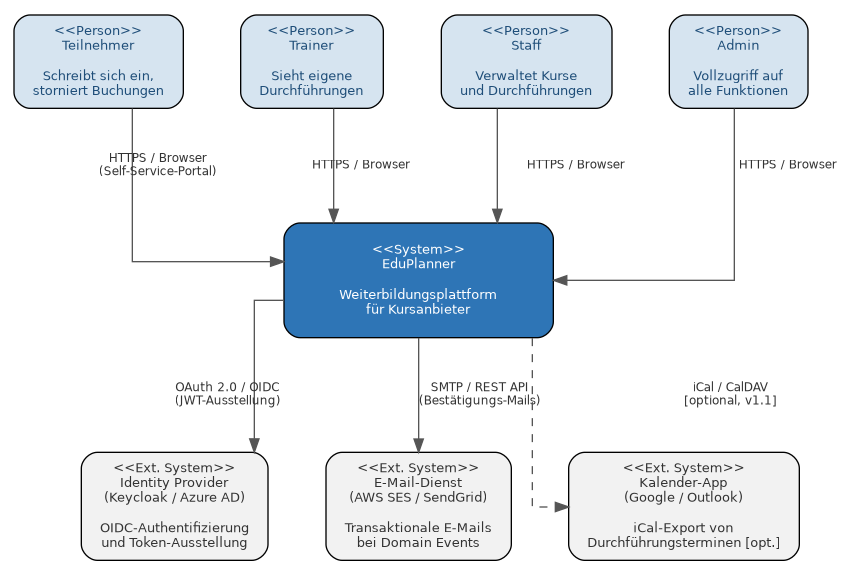
\includegraphics[width=\textwidth]{assets/context_diagram}
  \caption{\textit{C4 - Kontext Diagramm EduPlanner}}
  \label{fig:context_diagram}
\end{figure}

\subsection{Technischer Kontext}

\emph{Diagrammtyp: C4 Container Diagram.} Schichten:
\begin{enumerate}[leftmargin=2em]
  \item \textbf{Client:}
  Angular~SPA oder Vue.js~SPA (TypeScript) im Browser.
  \item \textbf{API Gateway:}
  Spring Cloud Gateway oder NGINX --
  TLS-Terminierung, Rate-Limiting, JWT-Weiterleitung.
  \item \textbf{Services:}
  catalog, scheduling, registration, notification,
  identity -- je in eigenem Kubernetes-Pod.
  \item \textbf{Datenhaltung:}
  Je eine PostgreSQL-Datenbank pro Service;
  RabbitMQ für asynchrone Events.
\end{enumerate}


\subsubsection{Technische Protokolle}

\begin{tabularx}{\textwidth}{L{4cm} L{2.8cm} X}
  \rowcolor{tableheader}
  \color{white}\textbf{Verbindung} & \color{white}\textbf{Protokoll} & \color{white}\textbf{Bemerkung} \\
  SPA $\to$ API Gateway & HTTPS / TLS & Port 443; REST APIs via JSON \\
  \rowcolor{tablegrey}
  Gateway $\to$ Services & HTTP / JSON & Internes K8s-Netzwerk; JWT-Header-Propagierung \\
  Services $\to$ DB & JDBC & PostgreSQL-Protokoll; Port 5432 \\
  \rowcolor{tablegrey}
  Services $\to$ RabbitMQ & AMQP & Port 5672; asynchrone Domain Events \\
  System $\to$ E-Mail & SMTP/REST & Verschlüsselt via STARTTLS oder REST-API \\
  \rowcolor{tablegrey}
  System $\to$ IdP & OIDC/OAuth~2.0 & HTTPS-Endpunkte für Token-Validation und UserInfo \\
  API-Spezifikation & OpenAPI~3.1.0 & Contract-First: Spec in \texttt{openapi/}\allowbreak \texttt{eduplanner-}\allowbreak \texttt{api.yaml};
  Swagger~UI je Service unter \texttt{/swagger-ui/index.html};
  vollständige Übersicht in Anhang~D (ADR-011). \\
\end{tabularx}

\subsection{Systemabgrenzung (Out-of-Scope)}

\begin{reviewbox}[Systemgrenze in einem Satz]
EduPlanner verwaltet Kurskatalog, Durchführungsplanung, Einschreibung,
Benachrichtigung und Identitätsanbindung -- \textbf{nicht} aber
Lerninhalte, Zahlungsflüsse oder die Passwortverwaltung der Nutzer.
\end{reviewbox}

Was EduPlanner \textbf{nicht} leistet (Explizite Abgrenzung nach arc42~v9):

\begin{tabularx}{\textwidth}{L{4cm} X}
  \rowcolor{tableheader}
  \color{white}\textbf{Nicht im Scope} &
  \color{white}\textbf{Begründung / Verweis} \\

  Lerninhalt (LMS) &
  EduPlanner verwaltet Kurse und Buchungen -- kein
  Moodle-Ersatz. Inhalte (Videos, Lernmaterial) liegen
  extern. LMS-Integration geplant für v2.0
  (Kap.~14). \\

  \rowcolor{tablegrey}
  Zahlungsabwicklung &
  Integration einer Zahlungsabwicklung wie z.\,B.\ Stripe
  erst in v2.0 (Kap.~14). Rechnungsstellung und
  Zahlungsflüsse sind kein MVP-Scope. \\

  Identity Management &
  Passwortverwaltung, MFA-Setup\footnotemark{} und
  User-Provisioning liegen vollständig beim externen
  IdP (ADR-003). \\

  \rowcolor{tablegrey}
  Videokonferenz / Streaming &
  Keine Integration von Zoom, MS-Teams o.\,ä.\
  Durchführungen können physisch oder extern gelinkt
  sein. \\

  Multi-Tenancy (v1.0) &
  Kursanbieter-Mandantentrennung erst ab v2.0
  (ADR-008, TS4). \\

  \rowcolor{tablegrey}
  Mobile App &
  Native iOS/Android-App erst in v2.0. v1.0: Responsive
  Web via gegebene SPA (Angular oder Vue.js). \\
\end{tabularx}

\footnotetext{%
  \textbf{MFA -- Multi-Factor Authentication}
  (Mehr-Faktor-Authentifizierung). Bei MFA muss sich ein
  Benutzer mit mindestens zwei unabhängigen Faktoren ausweisen,
  z.\,B.\ Passwort (Wissen) und Einmalcode per
  Authenticator-App (Besitz). \textbf{MFA-Setup} bezeichnet
  die erstmalige Einrichtung dieser zusätzlichen Faktoren --
  etwa das Verknüpfen einer Authenticator-App oder das
  Hinterlegen einer Mobilnummer für SMS-Codes. Im Kontext
  von EduPlanner liegt dieser gesamte Prozess beim externen
  Identity Provider und ist daher nicht Teil des eigenen
  Funktionsumfangs.%
}

